\documentclass[letterpaper,10pt]{article}
\usepackage[top=2cm, bottom=1.5cm, left=1cm, right=1cm]{geometry}
\usepackage{amsmath, amssymb, amsthm, graphicx}
\usepackage{fancyhdr}
\pagestyle{fancy}

\lhead{\today}
\chead{MATH498- Spatial Processes in Biology}
\rhead{Justin Hood}

\newcommand{\Z}{\mathbb{Z}}
\newcommand{\Q}{\mathbb{Q}}

\begin{document}
\begin{description}
\item[1.]\hfill \\
We consider the table of molecular weights and diffusion coefficients. Our rule of thumb for computing D from M is $D\approx M^{-1/3}$. Plotting the table on a log-log plot yields the result below.
\begin{center}
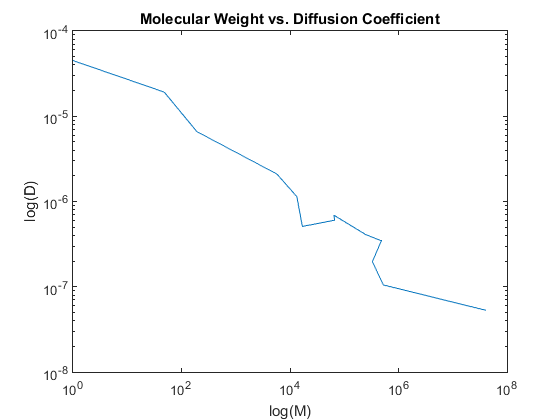
\includegraphics{pureplot.png}
\end{center}
We note that the plot is linear with values decreasing as M increases, as expected. Given that we can assume the data is proportional by the rule of thumb, we consider a line of best fit to be of the form,
\[D=beta_1M^{-\frac{1}{3}}+\beta_2\]
Using a linear fitting method, I determined the coefficients to be,
\begin{align*}
\beta_1 &\approx 4.779\times 10^{-5}\\
\beta_2 &\approx 1.399\times 10^{-7}
\end{align*}
Plotting the resultant line over the data yields the following result; which, from a purely visual inspection seems to support the rule of thumb as being accurate.
\begin{center}
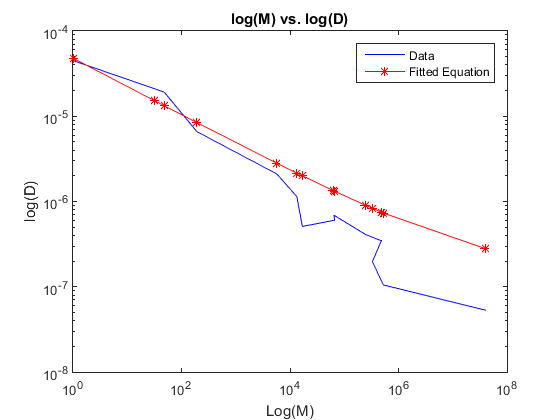
\includegraphics{bestfit.png}
\end{center}
In order to further validify the rule of thumb, we consider the slope of a line of best fit when we take the log of both sides. In this case, we construct a relation that looks like,
\[log(D)\approx \frac{-1}{3}log(M)\]
From this, we are able to see that a line of best fit should have a slope of $\frac{-1}{3}$. After running a model fit in R, I found that the best fit coefficient was $-.4274$. Plotting the resultant line over the data, we arrive at the following plot, further confirming our suspicions about the validity of the rule of thumb.
\begin{center}
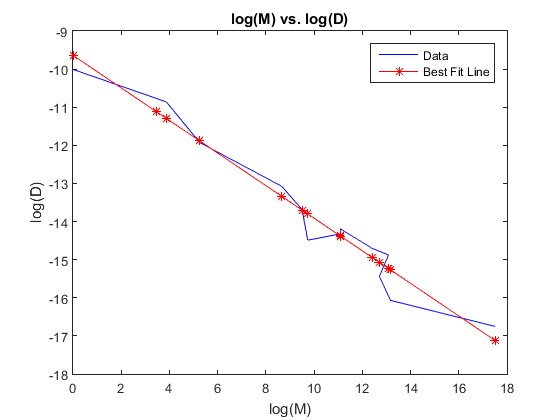
\includegraphics{best.png}
\end{center}
\item[2.] \hfill \\
We consider the area of a small intestine varying in time governed by,
\[A(x,t)=\frac{a}{2}\big[2+\cos(x-vt)\big]\]
Where $v$ is a constant.\\
To write the equation of balance for the concentration $c(x,t)$, we first consider the known conservation equation for 1-D,
\[\frac{\partial}{\partial t}[c(x,t)A(x,t)]=-\frac{\partial}{\partial x}[J(x,t)A(x,t)]\pm \sigma(x,t)A(x,t)\]
Where $J$ is the flux through the cross-sectional area $A$ at position $x$ and time $t$, and $\sigma$ is the local rate of creation/destruction of particles.
We now substitute into the equation, our known value fo A,
\[\frac{\partial}{\partial t}[c(x,t)(\frac{a}{2}\big[2+\cos(x-vt)\big])]=-\frac{\partial}{\partial x}[J(x,t)(\frac{a}{2}\big[2+\cos(x-vt)\big])]\pm \sigma(x,t)(\frac{a}{2}\big[2+\cos(x-vt)\big])\]
Using the product rule to expand both sides, we arrive at,
\[\frac{\partial c}{\partial t}(\frac{a}{2}\big[2+\cos(x-vt)\big])+c(\frac{-av}{2}\big[-\sin(x-vt)\big])\]
on the left hand side, and
\[-\frac{\partial J}{\partial x}(\frac{a}{2}\big[2+\cos(x-vt)\big])+J(\frac{a}{2}\big[-\sin(x-vt)\big])\pm \sigma (\frac{a}{2}\big[2+\cos(x-vt)\big])\]
Simplifying, and solving for $\frac{\partial c}{\partial t}$, we get,
\[\frac{\partial c}{\partial t}=-\frac{\partial J}{\partial x}\pm \sigma + \frac{(J-vc)\sin(x-vc)}{2+\cos(x-vt)}\]
Thus, we have our balance for $c$.\\
We now consider a constant flux of material, and an absorption rate proportional to concentration. Thus, we have
\begin{align*}
J&=1\\
\sigma&=-\alpha c
\end{align*} 
Substituting into the derived balance equation, we get,
\[\frac{\partial c}{\partial t}=-\alpha c+ \frac{(1-vc)\sin(x-vc)}{2+\cos(x-vt)}\]
Thus we have updated the force balance.\\
In a similar way, we consider $J=\sigma=0$.  Substituting into the derived balance yields,
\[\frac{\partial c}{\partial t}=\frac{(vc)\sin(x-vc)}{2+\cos(x-vt)}\]
This value is not necessarily zero, and thus, we see that the concentration will continue to change regardless.
\item[3.] \hfill \\
We consider the function,
\[p(x,t)=\frac{1}{\sqrt{4\pi Dt}}e^{-\frac{x^2}{4Dt}}\]
and the related integral, 
\[\int_{-\infty}^{\infty}p(x,t)dx\]
We solve the integral, by considering the new variable and differential,
\begin{align*}
u&=\frac{x}{\sqrt{4Dt}}\\
dx&=\sqrt{4Dt}du
\end{align*}
Substituting, we arrive at the following solution,
\begin{align*}
\int_{-\infty}^{\infty}p(x,t)dx&=\frac{1}{\sqrt{4\pi Dt}}\int_{-\infty}^{\infty}e^{-\frac{x^2}{4Dt}}dx\\
&=\frac{1}{\sqrt{4\pi Dt}}\int_{-\infty}^{\infty}e^{-u^2}\sqrt{4Dt}du\\
&=\frac{1}{\sqrt{\pi}}\int_{-\infty}^{\infty}e^{-u^2}du\\
&=\frac{\sqrt{\pi}}{\sqrt{\pi}}\\
&=1
\end{align*}
Thus, we see that the integral evaluates to one for all time.\
\item[6.]\hfill\\
We consider the balance equation for an arbitrary box with concentration $c_i$,
\[\frac{\partial c_i}{\partial t}=\frac{1}{(\Delta x)^2}\bigg(\lambda_{i-1}c_{i-1}+\lambda_{i+1}c_{i+1}-2\lambda_ic_i\bigg)\]
We now define the expression, $J_i=\lambda_ic_i$ and re-write the equation,
\[\frac{\partial c}{\partial t}=\frac{1}{(\Delta x)^2}\bigg(J_{i-1}-2J_i+J_{i+1}\bigg)\]
Noting the second order difference equation, we re-write the equation, allowing the relation to hold for all boxes,
\[\frac{\partial c}{\partial t}=\frac{\partial^2 J}{\partial x^2}\]
Simplifying into conservation form, we arrive at,
\[\frac{\partial c}{\partial t}=\frac{\partial}{\partial x}\bigg(\frac{\partial J}{\partial x}\bigg)=\frac{\partial}{\partial x}\bigg(\frac{\partial}{\partial x}\big(\lambda c\big)\bigg)\]
Where the expressions in the parentheses are the flux terms.
\item[7.]\hfill\\
We consider the balance equation for an arbitrary box with concentration $c_i$,
\[\frac{\partial c_i}{\partial t}=\frac{1}{(\Delta x)^2}\bigg(\lambda_{(i-1)+1}c_{i-1}+\lambda_{(i+1)-1}c_{i+1}-lambda_{i+1}c_i-l\lambda_{i-1}c_i\bigg)\]
We then add and subtract the value of $\frac{2\lambda_ic_i}{(\Delta x)^2}$ to the above equation and re-arrange to arrive at,
\[\frac{\partial c_i}{\partial t}=\frac{1}{(\Delta x)^2}\bigg(\lambda_{i}\big(c_{i-1}-2c_i+c_{i+1}\big)-c_i\big(\lambda_{i-1}-2\lambda_i+\lambda_{i+1}\big)\bigg)\]
We may now see that there are two second order difference equations in this equation, and we now write them as such, and allow the relation to hold over all boxes.
\[\frac{\partial c}{\partial t}=\lambda\frac{\partial^2 c}{\partial x^2}-c\frac{d^2 \lambda}{dx^2}+O(\Delta x^2)\]
We note that lambda is defined as only a function of x, and as such, we may simplify the partial into an ordinary derivative. Putting this into conservation form, we arrive at,
\[\frac{\partial c}{\partial t}=\frac{\partial}{\partial x}\bigg(\lambda(x)\frac{\partial c}{\partial x}-c\frac{d\lambda}{dx}\bigg)\]
Here, the flux term is the inside of the parentheses.
\end{description}


\end{document}
